% =============================================================================
% Data Pipeline and Model Construction — Section Draft
% =============================================================================
% Compile with:  pdflatex section_data_pipeline.tex
%                bibtex   section_data_pipeline
%                pdflatex section_data_pipeline.tex  (x2)
% =============================================================================

\documentclass[11pt,a4paper]{article}

% ---------- packages ----------
\usepackage[utf8]{inputenc}
\usepackage[T1]{fontenc}
\usepackage{amsmath,amssymb,amsthm,mathtools}
\usepackage{bm}
\usepackage{booktabs}
\usepackage{graphicx}
\usepackage[dvipsnames]{xcolor}
\usepackage{hyperref}
\usepackage{cleveref}
\usepackage{microtype}
\usepackage{enumitem}
\usepackage{geometry}
\usepackage{caption}
\usepackage{subcaption}
\usepackage{algorithm}
\usepackage{algpseudocode}
\usepackage{tikz}
\usetikzlibrary{arrows.meta,positioning,shapes.geometric,fit,backgrounds,calc}

\geometry{margin=2.5cm}
\hypersetup{colorlinks=true,linkcolor=MidnightBlue,citecolor=MidnightBlue,urlcolor=MidnightBlue}

% ---------- notation shortcuts ----------
\newcommand{\R}{\mathbb{R}}
\newcommand{\N}{\mathbb{N}}
\newcommand{\indicator}{\mathbb{1}}
\newcommand{\calT}{\mathcal{T}}
\newcommand{\calG}{\mathcal{G}}
\newcommand{\calE}{\mathcal{E}}
\newcommand{\calN}{\mathcal{N}}
\newcommand{\calI}{\mathcal{I}}
\newcommand{\bx}{\bm{x}}
\newcommand{\bP}{\bm{P}}
\newcommand{\bA}{\bm{A}}
\newcommand{\bX}{\bm{X}}
\newcommand{\bM}{\bm{M}}
\newcommand{\bPhi}{\bm{\Phi}}
\DeclareMathOperator*{\argmin}{arg\,min}

\title{%
  Data Pipeline and Model Construction for \\
  Graph--Temporal P\&L Prediction of Exotic Derivatives%
}
\author{DRAFT --- NOT FOR DISTRIBUTION}
\date{\today}

% =============================================================================
\begin{document}
\maketitle

% =============================================================================
\section{Introduction}\label{sec:intro}
% =============================================================================

The accurate prediction of daily profit-and-loss (P\&L) for portfolios of
exotic derivative instruments constitutes a challenging regression problem at
the intersection of financial engineering and representation learning.  Unlike
vanilla options, whose sensitivities are well characterised by low-order Greeks,
exotic payoffs exhibit path dependence, discontinuous barrier events, and
complex cross-instrument interactions that resist closed-form approximation.
Traditional risk systems rely on Monte Carlo re-valuation, which is
computationally expensive and provides limited scope for intra-day,
portfolio-wide forecasting.

In this work we develop a neural architecture that ingests both the
\emph{structural} relationships between trades---encoded as a sparse
graph---and the \emph{temporal} dynamics of their mark-to-market
valuations---encoded as multivariate time series.  A prerequisite for this
architecture is a data pipeline that transforms raw market data and trade-level
bookings into a set of well-conditioned tensor inputs.  The design of this
pipeline is non-trivial: the raw data is heterogeneous, high-dimensional,
irregularly observed, and heavy-tailed.

This section describes the end-to-end pipeline, which comprises five stages:
%
\begin{enumerate}[label=(\roman*),nosep]
  \item \textbf{Elementary P\&L construction} (\Cref{sec:pnl}):
        extraction and standardisation of per-trade daily P\&L series.
  \item \textbf{Trade graph construction} (\Cref{sec:graph}):
        formation of a sparse $k$-nearest-neighbour graph over the trade
        universe in attribute space.
  \item \textbf{Attribute encoding} (\Cref{sec:attributes}):
        mapping of heterogeneous trade descriptors into fixed-length feature
        vectors via learned embeddings and normalisation.
  \item \textbf{Dimensionality reduction} (\Cref{sec:dimred}):
        projection of the P\&L matrix onto a truncated orthogonal basis that
        preserves the dominant modes of portfolio covariance.
  \item \textbf{Model input assembly} (\Cref{sec:assembly}):
        packaging of the above outputs into the structured tensor collection
        consumed by the model.
\end{enumerate}
%
Each stage is designed to be modular: the graph construction, attribute
encoding, and dimensionality reduction may be independently reconfigured
without altering the model architecture, thereby facilitating rapid
experimentation across asset classes and portfolio compositions.  A schematic
overview of the full pipeline is provided in~\Cref{fig:pipeline-overview}.

\begin{figure*}[t]
  \centering
  \resizebox{\textwidth}{!}{%
  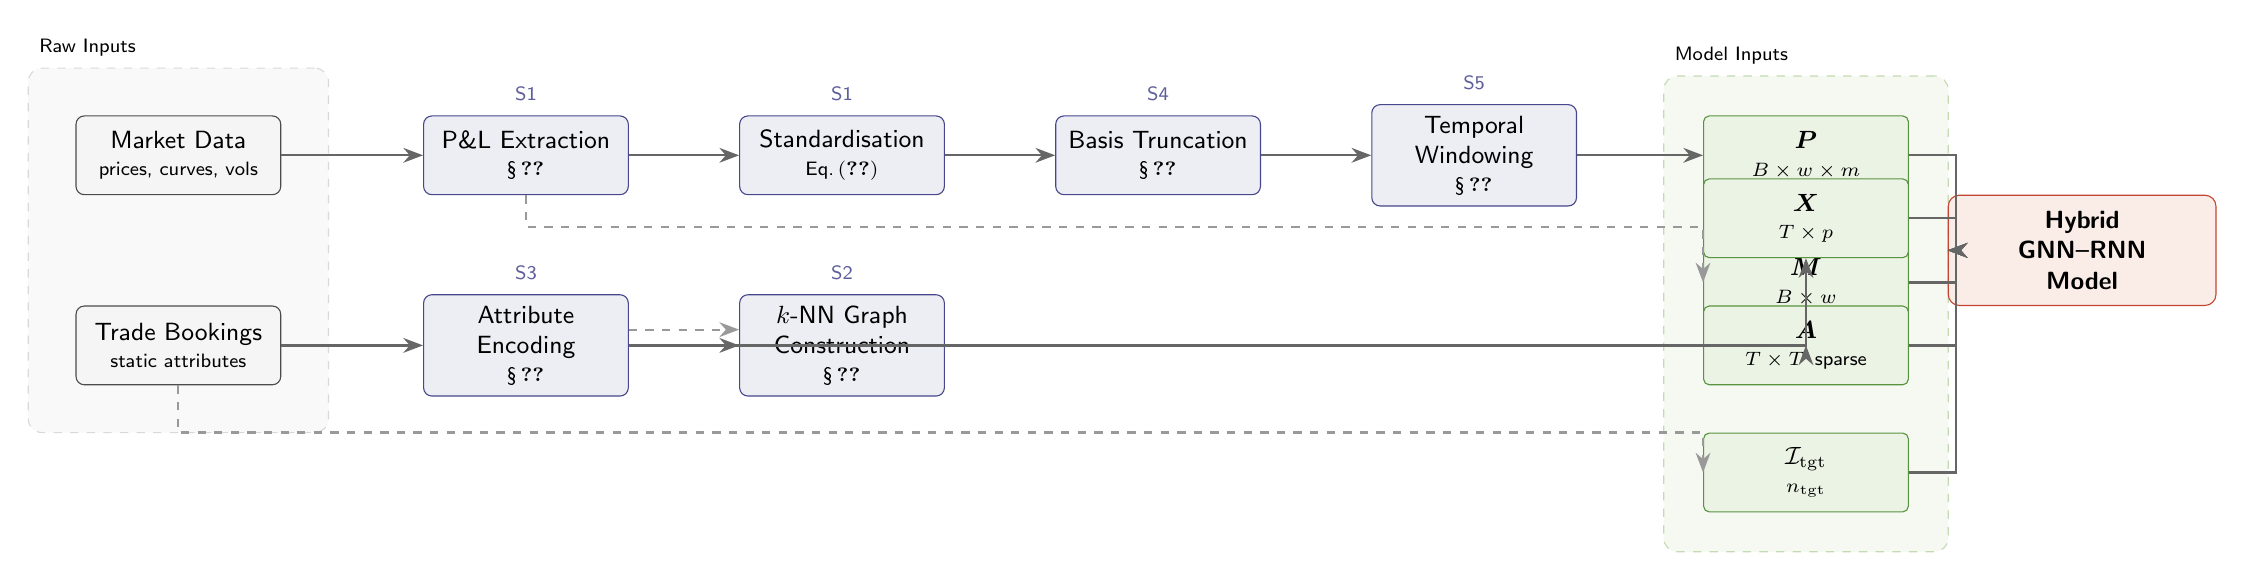
\begin{tikzpicture}[
    % --- node styles ---
    source/.style={
      rectangle, rounded corners=3pt, draw=black!70, fill=gray!8,
      minimum height=10mm, minimum width=26mm, align=center,
      font=\small\sffamily},
    process/.style={
      rectangle, rounded corners=3pt, draw=MidnightBlue!80,
      fill=MidnightBlue!8, minimum height=10mm, minimum width=26mm,
      align=center, font=\small\sffamily},
    tensor/.style={
      rectangle, rounded corners=2pt, draw=OliveGreen!80,
      fill=OliveGreen!8, minimum height=10mm, minimum width=26mm,
      align=center, font=\small\sffamily},
    model/.style={
      rectangle, rounded corners=4pt, draw=BrickRed!80,
      fill=BrickRed!6, minimum height=14mm, minimum width=34mm,
      align=center, font=\small\sffamily\bfseries},
    stage/.style={
      font=\scriptsize\sffamily\color{MidnightBlue!70}, above=1pt},
    arr/.style={-{Stealth[length=2.5mm]}, thick, draw=black!60},
    darr/.style={-{Stealth[length=2.5mm]}, thick, draw=black!40, dashed},
    every node/.append style={inner sep=4pt},
  ]

  % ============== RAW INPUTS (left column) ==============
  \node[source] (mktdata)  {Market Data\\[-1pt]{\scriptsize prices, curves, vols}};
  \node[source, below=14mm of mktdata] (bookings) {Trade Bookings\\[-1pt]{\scriptsize static attributes}};

  % ============== ELEMENTARY PNL BRANCH (top) ==============
  \node[process, right=18mm of mktdata] (extract) {P\&L Extraction\\[-1pt]{\scriptsize \S\,\ref{sec:pnl}}};
  \node[process, right=14mm of extract] (standardise) {Standardisation\\[-1pt]{\scriptsize Eq.\,\eqref{eq:standardise}}};
  \node[process, right=14mm of standardise] (dimred) {Basis Truncation\\[-1pt]{\scriptsize \S\,\ref{sec:dimred}}};
  \node[process, right=14mm of dimred] (window) {Temporal\\Windowing\\[-1pt]{\scriptsize \S\,\ref{sec:assembly:windowing}}};

  % ============== ATTRIBUTE BRANCH (bottom) ==============
  \node[process, right=18mm of bookings] (encode) {Attribute\\Encoding\\[-1pt]{\scriptsize \S\,\ref{sec:attributes}}};
  \node[process, right=14mm of encode] (graph) {$k$-NN Graph\\Construction\\[-1pt]{\scriptsize \S\,\ref{sec:graph}}};

  % ============== OUTPUT TENSORS (right) ==============
  \node[tensor, right=16mm of window] (Ptensor) {$\bP$\\[-1pt]{\scriptsize $B \times w \times m$}};
  \node[tensor, below=6mm of Ptensor] (Mmask) {$\bM$\\[-1pt]{\scriptsize $B \times w$}};

  \node[tensor] at (Ptensor |- graph) (Atensor) {$\bA$\\[-1pt]{\scriptsize $T \times T$\, sparse}};
  \node[tensor, above=6mm of Atensor] (Xtensor) {$\bX$\\[-1pt]{\scriptsize $T \times p$}};
  \node[tensor, below=6mm of Atensor] (Itarget) {$\calI_{\mathrm{tgt}}$\\[-1pt]{\scriptsize $n_{\mathrm{tgt}}$}};

  % ============== MODEL (far right) ==============
  \node[model, right=18mm of $(Mmask)!0.5!(Xtensor)$] (model)
    {Hybrid\\GNN--RNN\\Model};

  % ============== ARROWS: data flow ==============
  \draw[arr] (mktdata)     -- (extract);
  \draw[arr] (extract)     -- (standardise);
  \draw[arr] (standardise) -- (dimred);
  \draw[arr] (dimred)      -- (window);
  \draw[arr] (window)      -- (Ptensor);

  \draw[arr] (bookings)    -- (encode);
  \draw[arr] (encode)      -- (graph);
  \draw[arr] (graph)       -| (Atensor);
  \draw[arr] (encode)      -| (Xtensor);

  % mask comes from extraction
  \draw[darr] (extract.south) -- ++(0,-4mm) -| (Mmask.west);

  % target indices from bookings
  \draw[darr] (bookings.south) -- ++(0,-6mm) -| (Itarget.west);

  % attribute matrix also feeds graph construction
  \draw[darr] ([yshift=2mm]encode.east) -- ([yshift=2mm]graph.west);

  % tensors into model
  \draw[arr] (Ptensor.east)  -- ++(6mm,0) |- (model.west);
  \draw[arr] (Mmask.east)    -- ++(6mm,0) |- (model.west);
  \draw[arr] (Xtensor.east)  -- ++(6mm,0) |- (model.west);
  \draw[arr] (Atensor.east)  -- ++(6mm,0) |- (model.west);
  \draw[arr] (Itarget.east)  -- ++(6mm,0) |- (model.west);

  % ============== STAGE LABELS ==============
  \node[stage] at (extract.north)     {S1};
  \node[stage] at (standardise.north) {S1};
  \node[stage] at (encode.north)      {S3};
  \node[stage] at (graph.north)       {S2};
  \node[stage] at (dimred.north)      {S4};
  \node[stage] at (window.north)      {S5};

  % ============== BACKGROUND GROUPS ==============
  \begin{scope}[on background layer]
    \node[fit=(mktdata)(bookings), inner sep=6mm, rounded corners=5pt,
          fill=gray!5, draw=gray!30, dashed,
          label={[font=\scriptsize\sffamily,anchor=south west]north west:Raw Inputs}] {};
    \node[fit=(Ptensor)(Mmask)(Xtensor)(Atensor)(Itarget),
          inner sep=5mm, rounded corners=5pt,
          fill=OliveGreen!4, draw=OliveGreen!25, dashed,
          label={[font=\scriptsize\sffamily,anchor=south west]north west:Model Inputs}] {};
  \end{scope}

  \end{tikzpicture}%
  }% end resizebox
  \caption{%
    End-to-end data pipeline from raw market data and trade bookings to the
    structured tensor inputs consumed by the Hybrid GNN--RNN architecture.
    Solid arrows indicate tensor data flow; dashed arrows indicate
    configuration dependencies or secondary outputs.  Stage labels
    S1--S5 correspond to
    \Cref{sec:pnl,sec:graph,sec:attributes,sec:dimred,sec:assembly},
    respectively.  Tensor shapes are annotated on each output node, where
    $T$~is the number of trades, $B$~the batch size, $w$~the window length,
    $m$~the reduced basis dimension, $p$~the attribute feature dimension, and
    $n_{\mathrm{tgt}}$~the number of target trades.%
  }
  \label{fig:pipeline-overview}
\end{figure*}


% =============================================================================
\section{Elementary P\&L Construction}\label{sec:pnl}
% =============================================================================

\subsection{Extraction and temporal alignment}\label{sec:pnl:extract}

Let $\calT = \{1,\dotsc,T\}$ denote the universe of $T$ live trades observed
over $S$ business days indexed by $t \in \{1,\dotsc,S\}$.  For each trade~$i$,
the front-office risk system provides a daily mark-to-market P\&L value
$\tilde{p}_{i,t}$, computed as the change in the instrument's net present
value between consecutive close-of-business snapshots:
%
\begin{equation}\label{eq:raw-pnl}
  \tilde{p}_{i,t}
  \;=\;
  \mathrm{NPV}_i(t) - \mathrm{NPV}_i(t-1),
  \qquad
  i \in \calT,\;
  t \in \{1,\dotsc,S\}.
\end{equation}
%
The resulting \emph{elementary P\&L matrix}
$\tilde{\bP} \in \R^{T \times S}$ is the foundational data object from which
all temporal features are derived.

In practice, not every trade is live for the entire observation window.
Instruments booked after the start of the window, or maturing before its end,
produce incomplete rows.  We handle this by zero-padding the missing entries
and constructing a binary availability mask
$\bM \in \{0,1\}^{T \times S}$:
%
\begin{equation}\label{eq:mask}
  M_{i,t}
  \;=\;
  \begin{cases}
    1 & \text{if trade } i \text{ is live on day } t, \\
    0 & \text{otherwise}.
  \end{cases}
\end{equation}
%
The mask is propagated downstream to prevent the model from treating padding
as informative signal.  This treatment follows the masked sequence modelling
paradigm introduced in the natural language processing literature
\cite{devlin2019bert} and subsequently adapted to irregularly observed
clinical and financial time series \cite{che2018recurrent}.


\subsection{Trade-level standardisation}\label{sec:pnl:standardise}

Raw elementary P\&L exhibits two properties that are problematic for
gradient-based optimisation.  First, the marginal distributions are
heavy-tailed, reflecting the non-linear payoff profiles of exotic instruments:
barrier knock events, fixing resets, and early exercise can produce daily P\&L
realisations several standard deviations from the mean.  Second, the variance
is \emph{heterogeneous} across instrument types---a deep out-of-the-money
barrier option may exhibit daily fluctuations orders of magnitude smaller than
an at-the-money vanilla on the same underlying \cite{cont2001empirical}.

Both properties violate the implicit assumptions of common loss functions and
optimisers, leading to poorly conditioned gradients and slow convergence.  We
address this via a trade-level location-scale standardisation:
%
\begin{equation}\label{eq:standardise}
  \bar{p}_{i,t}
  \;=\;
  \frac{\tilde{p}_{i,t} - \hat{\mu}_i}{\hat{\sigma}_i + \epsilon},
\end{equation}
%
where $\hat{\mu}_i$ and $\hat{\sigma}_i$ are robust estimates of the
$i$\textsuperscript{th} trade's central tendency and dispersion, computed over
a trailing calibration window of length~$W_{\mathrm{cal}}$, and
$\epsilon > 0$ is a small constant that prevents degenerate scaling for trades
with near-zero P\&L variance (\emph{e.g.}, deeply out-of-the-money positions
approaching maturity).  The use of \emph{robust} estimators---rather than
simple sample moments---provides resilience to the outliers that routinely
arise in exotic derivative portfolios.

The standardised matrix $\bar{\bP} \in \R^{T \times S}$ has approximately
zero mean and unit variance per trade, enabling the recurrent network stream
to operate in a numerically well-conditioned regime irrespective of the
heterogeneous composition of the portfolio.

\begin{figure}[t]
  \centering
  % ---- Replace with synthetic plots ----
  \fbox{\parbox{0.92\linewidth}{\centering\vspace{2.5cm}%
    \textsc{Figure Placeholder}\\[4pt]
    (a) Raw P\&L histograms: heavy tails, heteroscedastic scale.\\
    (b) Post-standardisation: approximately unit-variance marginals.
  \vspace{2.5cm}}}
  \caption{%
    Distributional effect of trade-level standardisation on a synthetic
    portfolio of 500 trades sampled from a mixture of Student-$t$
    distributions with degrees of freedom $\nu \in \{3,5,10\}$ and scale
    parameters spanning three orders of magnitude.%
  }
  \label{fig:standardisation}
\end{figure}


% =============================================================================
\section{Trade Graph Construction}\label{sec:graph}
% =============================================================================

\subsection{Motivation and design rationale}\label{sec:graph:motivation}

The graph neural network stream of the architecture requires an explicit
relational structure over the trade universe.  Unlike domains in which the
graph is given \emph{a~priori}---molecular bond graphs, social networks, road
networks---the trade graph must be \emph{constructed} from available data.  The
design of this graph constitutes a critical modelling decision, as it
encodes the inductive bias governing which instruments are permitted to
exchange information during message passing.

We adopt a $k$-nearest-neighbour ($k$-NN) construction in the trade attribute
space, motivated by the empirical observation that trades sharing structural
characteristics---common underlying assets, proximate moneyness, overlapping
tenor---exhibit correlated P\&L dynamics.  This approach is related to the
broader literature on learning graph structure from data
\cite{kipf2018neural,franceschi2019learning}, though we opt for a fixed,
pre-computed graph rather than a jointly learned topology, as the latter
introduces a costly bilevel optimisation that is difficult to stabilise at the
portfolio scales we consider ($T \sim 10^3$--$10^4$).


\subsection{Construction procedure}\label{sec:graph:construction}

Let $\bX \in \R^{T \times p}$ denote the attribute matrix described in
\Cref{sec:attributes}.  For each trade~$i$, we compute a pairwise affinity
score $s(i,j)$ to every other trade $j \in \calT$ and retain the $k$~trades
with the highest affinity as neighbours, forming the neighbour set
$\calN_k(i)$.  The affinity function operates over a mixed feature space
comprising both categorical and continuous attributes; the precise formulation
is domain-specific and is not detailed here.

The resulting directed graph $\calG = (\calT, \calE)$ has
$|\calE| = T \cdot k$ edges.  We form the weighted adjacency matrix
$\bA \in \R^{T \times T}$ by row-normalising the affinity scores:
%
\begin{equation}\label{eq:adjacency}
  A_{ij}
  \;=\;
  \frac{
    s(i,j)\;\indicator\bigl[j \in \calN_k(i)\bigr]
  }{
    \displaystyle\sum_{j' \in \calN_k(i)} s(i,j')
  }.
\end{equation}
%
Row normalisation ensures that the mean aggregation operator in the
GraphSAGE message-passing step \cite{hamilton2017inductive} computes a
properly weighted average over neighbours, and that isolated or sparsely
connected nodes do not produce unbounded feature magnitudes.

The adjacency matrix is stored in sparse coordinate (COO) format.  For a
portfolio of $T = 2{,}000$ trades with $k = 30$, the sparse representation
stores $6 \times 10^4$ non-zero entries in lieu of the $4 \times 10^6$
elements required by a dense representation---a reduction that is essential
for memory-efficient training and inference.

\begin{figure}[t]
  \centering
  % ---- Replace with synthetic graph visualisation ----
  \fbox{\parbox{0.92\linewidth}{\centering\vspace{3cm}%
    \textsc{Figure Placeholder}\\[4pt]
    Force-directed layout of a synthetic $k$-NN graph\\
    ($T\!=\!200$, $k\!=\!10$, four product families).
  \vspace{3cm}}}
  \caption{%
    Illustrative $k$-NN trade graph generated from four isotropic Gaussian
    clusters in $\R^2$, each representing a distinct product family.  Node
    colour indicates cluster membership.  Intra-cluster connectivity is
    dense, reflecting high attribute-space affinity, while inter-cluster edges
    arise from trades at cluster boundaries with shared characteristics.%
  }
  \label{fig:trade-graph}
\end{figure}


\subsection{Receptive field and connectivity trade-offs}%
\label{sec:graph:properties}

The neighbour count~$k$ controls the trade-off between locality and
connectivity.  Small~$k$ yields a sparse graph that preserves fine-grained
structural distinctions but may under-connect instruments sharing indirect
relationships through intermediary trades.  Large~$k$ yields a denser graph
that enables broader information propagation at the cost of diluting the
neighbourhood signal with less relevant trades.

In a multi-layer GNN of depth~$L$, the effective receptive field of each node
encompasses its $L$-hop neighbourhood, the size of which grows as
$\mathcal{O}(k^L)$ in the worst case \cite{xu2019powerful,alon2021bottleneck}.
Consequently, even moderate values of~$k$ permit the model to aggregate
information from structurally distant trades when multiple message-passing
layers are employed.  We observe empirically that the optimal~$k$ varies with
portfolio composition: concentrated books with few product types favour smaller
values, whereas diversified multi-asset portfolios benefit from larger~$k$ to
capture cross-asset-class dependencies.


% =============================================================================
\section{Attribute Encoding}\label{sec:attributes}
% =============================================================================

\subsection{Feature taxonomy}\label{sec:attributes:taxonomy}

Each trade $i \in \calT$ is described by a vector of static attributes drawn
from the trade booking system and the risk engine.  These attributes partition
naturally into two categories:
%
\begin{itemize}[nosep]
  \item \textbf{Categorical features.}  Discrete identifiers such as product
    type (vanilla, barrier, Asian, autocallable, \ldots), currency pair,
    exchange venue, and counterparty classification.  These possess no natural
    ordering and may exhibit high cardinality.
  \item \textbf{Continuous features.}  Real-valued risk sensitivities
    (Greeks)---delta, gamma, vega, theta---and contractual quantities such as
    notional, moneyness, and time-to-maturity.  These are informative of the
    trade's local sensitivity to market factors but operate on heterogeneous
    scales and may exhibit non-stationarity (\emph{e.g.}, gamma increases
    sharply as a barrier is approached).
\end{itemize}
%
The precise choice of which attributes to include is a domain engineering
decision that depends on the asset class, the available data, and the risk
factors of interest \cite{hull2022options,glasserman2003monte}.  We emphasise
that the attribute set should be jointly informative for both the graph
construction (\Cref{sec:graph}) and the projection layer's $k$-NN transfer
mechanism, as both modules rely on attribute-space proximity to generalise
across instruments.


\subsection{Encoding strategy}\label{sec:attributes:encoding}

Categorical features are mapped to dense vectors via learned embedding
look-up tables, following established practice in deep learning for tabular
data \cite{guo2016entity,gorishniy2021revisiting}.  For a categorical feature
with vocabulary size~$V$, the embedding dimension is set to
$\min\!\bigl(d_{\max},\,\lceil V/2\rceil\bigr)$, where $d_{\max}$ is a
configurable upper bound that balances expressiveness against parameter count.

Continuous features are standardised using training-set statistics and
optionally Winsorised at the $c$\textsuperscript{th} percentile to mitigate
the influence of extreme realisations in the Greeks that arise during periods
of market stress.

The encoded categorical embeddings and standardised continuous features are
concatenated to form the per-trade feature vector
$\bx_i \in \R^p$, and the full attribute matrix
%
\begin{equation}\label{eq:attribute-matrix}
  \bX
  \;=\;
  \bigl[\bx_1;\;\bx_2;\;\dotsc;\;\bx_T\bigr]
  \;\in\; \R^{T \times p}
\end{equation}
%
serves as input to both the GNN stream (as node features) and the projection
layer (for $k$-NN-based generalisation to unseen trades).


% =============================================================================
\section{Dimensionality Reduction of the P\&L Basis}\label{sec:dimred}
% =============================================================================

\subsection{Motivation}\label{sec:dimred:motivation}

The standardised P\&L matrix $\bar{\bP} \in \R^{T \times S}$ may possess a
large temporal dimension, particularly when extended observation windows are
employed to capture slow-moving risk factors.  For a portfolio of $T = 500$
trades observed over $S = 500$ business days, the recurrent stream would
process sequences of length~500 per training window---computationally
expensive and susceptible to overfitting, given that the number of free
parameters in the recurrent layers scales linearly with the input dimension.

The feasibility of compression rests on a well-documented property of
derivative portfolios: the daily P\&L of even a large, heterogeneous book is
driven by a comparatively small number of market risk factors---equity spot
levels, implied volatility surface nodes, yield curve key rates---and the
instrument-level P\&L vectors lie approximately on a low-dimensional manifold
determined by the portfolio's aggregate factor exposures
\cite{cont2011statistical,litterman1991common}.  Empirically, the leading
10--30 eigenvalues of the P\&L covariance matrix typically account for 90--97\%
of the total variance, with the trailing eigenspace dominated by idiosyncratic
noise.


\subsection{Orthogonal basis truncation}\label{sec:dimred:truncation}

We exploit the low-rank structure by projecting $\bar{\bP}$ onto a truncated
orthogonal basis.  Let
%
\begin{equation}\label{eq:svd}
  \bar{\bP}
  \;=\;
  \bm{U}\,\bm{\Sigma}\,\bm{V}^\top
\end{equation}
%
denote the (economy) singular value decomposition of $\bar{\bP}$, where
$\bm{U} \in \R^{T \times r}$, $\bm{\Sigma} = \operatorname{diag}(\sigma_1,
\dotsc,\sigma_r)$ with $\sigma_1 \geq \sigma_2 \geq \dotsb \geq \sigma_r
\geq 0$, $\bm{V} \in \R^{S \times r}$, and $r = \min(T,S)$.  Define the
\emph{retained basis} $\bPhi = [\bm{v}_1,\dotsc,\bm{v}_m] \in \R^{S
\times m}$ comprising the leading $m$~right singular vectors.  The compressed
representation is then
%
\begin{equation}\label{eq:projection}
  \bP_{\mathrm{red}}
  \;=\;
  \bar{\bP}\;\bPhi
  \;\in\; \R^{T \times m}.
\end{equation}

The truncation order~$m$ is selected such that the retained fraction of the
total variance exceeds a prescribed threshold~$\tau$:
%
\begin{equation}\label{eq:tau}
  m
  \;=\;
  \min\biggl\{
    m' \in \N
    \;\bigg|\;
    \frac{\displaystyle\sum_{k=1}^{m'} \sigma_k^2}
         {\displaystyle\sum_{k=1}^{r}   \sigma_k^2}
    \;\geq\; \tau
  \biggr\}.
\end{equation}
%
We use the SVD of $\bar{\bP}$ directly, rather than forming the Gram matrix
$\bar{\bP}^\top\!\bar{\bP}$ and computing its eigendecomposition, to avoid
the squaring of condition numbers that can lead to loss of numerical precision
in the trailing singular values \cite{golub2013matrix}.

An alternative to the heuristic threshold~$\tau$ is the optimal hard threshold
of Gavish and Donoho~\cite{gavish2014optimal}, which provides a
distribution-free, asymptotically optimal truncation rule under the spiked
covariance model:
%
\begin{equation}\label{eq:gavish}
  m^{\star}
  \;=\;
  \#\bigl\{
    k : \sigma_k > \omega(\beta)\,\hat{\sigma}_{\mathrm{med}}
  \bigr\},
  \qquad
  \omega(\beta) = 0.56\,\beta^3 - 0.95\,\beta^2 + 1.82\,\beta + 1.43,
\end{equation}
%
where $\beta = T/S$ is the aspect ratio and
$\hat{\sigma}_{\mathrm{med}}$ is the median singular value.  In our
experiments both criteria yield similar truncation orders; we report results
under the variance-threshold criterion~\eqref{eq:tau} as it is more widely
familiar to practitioners.


\subsection{Basis selection diagnostics}\label{sec:dimred:diagnostics}

The choice of~$\tau$ (equivalently,~$m$) governs the trade-off between
information retention and regularisation.  We recommend inspecting the spectral
structure of $\bar{\bP}$ prior to fixing~$\tau$:
%
\begin{itemize}[nosep]
  \item \emph{Cumulative variance plot}:
    $\sum_{k=1}^{m'}\sigma_k^2 \big/ \sum_{k=1}^{r}\sigma_k^2$ versus~$m'$,
    with the threshold $\tau$ indicated by a horizontal reference line.
  \item \emph{Scree plot}:
    individual singular values $\sigma_k$ (log scale) versus~$k$, revealing
    the ``elbow'' that separates systematic from idiosyncratic modes.
  \item \emph{Reconstruction error}:
    $\lVert \bar{\bP} - \bar{\bP}\,\bPhi\,\bPhi^\top \rVert_F
    \big/ \lVert \bar{\bP} \rVert_F$
    versus~$m$, illustrating the diminishing returns of additional components.
\end{itemize}

\begin{figure}[t]
  \centering
  % ---- Replace with synthetic diagnostic plots ----
  \fbox{\parbox{0.92\linewidth}{\centering\vspace{3cm}%
    \textsc{Figure Placeholder}\\[4pt]
    (a) Cumulative explained variance vs.\ number of components $m$.\\
    (b) Scree plot of singular values (log scale).\\
    (c) Relative reconstruction error vs.\ $m$.
  \vspace{3cm}}}
  \caption{%
    Basis selection diagnostics for a synthetic covariance structure with
    singular values following a power-law decay
    $\sigma_k \propto k^{-\alpha/2}$, $\alpha = 1.5$, calibrated to
    reproduce the spectral decay rate observed in derivative portfolio
    P\&L matrices.  Dashed horizontal line in~(a) indicates
    $\tau = 0.95$, corresponding to $m = 23$ out of $S = 500$
    components.%
  }
  \label{fig:basis-diagnostics}
\end{figure}


% =============================================================================
\section{Model Input Assembly}\label{sec:assembly}
% =============================================================================

\subsection{Temporal windowing}\label{sec:assembly:windowing}

The compressed P\&L matrix $\bP_{\mathrm{red}} \in \R^{T \times m}$
represents the entire observation history as a single snapshot.  To form the
recurrent input, we extract overlapping windows of length~$w$ along the
temporal axis.  Each window constitutes one training sample: the model
observes the compressed P\&L dynamics over $w$~consecutive business days and
produces a prediction for the subsequent period.

Let $B$ denote the total number of such windows.  The recurrent input tensor
is
%
\begin{equation}\label{eq:recurrent-input}
  \bP \;\in\; \R^{B \times w \times m},
\end{equation}
%
where $P_{b,:,:}$ contains the $m$-dimensional compressed P\&L for the
$b$\textsuperscript{th} window.  The window length~$w$ and the stride between
consecutive windows are hyperparameters that control the trade-off between
temporal context and the number of training samples.


\subsection{Structured input collection}\label{sec:assembly:inputs}

The complete model input is a structured collection of five tensors, summarised
in \Cref{tab:inputs}.

\begin{table}[t]
  \centering
  \caption{%
    Model input tensors.  The adjacency matrix and attribute features are
    batch-invariant (shared across all $B$ training windows).%
  }
  \label{tab:inputs}
  \begin{tabular}{@{}llll@{}}
    \toprule
    \textbf{Symbol} & \textbf{Shape} & \textbf{Description} & \textbf{Source} \\
    \midrule
    $\bX$
      & $T \times p$
      & Encoded trade attributes
      & \Cref{sec:attributes} \\
    $\bP$
      & $B \times w \times m$
      & Windowed, basis-reduced P\&L
      & \Cref{sec:dimred} \\
    $\bA$
      & $T \times T$ (sparse)
      & Row-normalised $k$-NN adjacency
      & \Cref{sec:graph} \\
    $\calI_{\mathrm{tgt}}$
      & $n_{\mathrm{tgt}}$
      & Target trade indices
      & Portfolio definition \\
    $\bM$
      & $B \times w$
      & Binary availability mask
      & \Cref{sec:pnl} \\
    \bottomrule
  \end{tabular}
\end{table}

The graph~$\bA$ and attribute matrix~$\bX$ are \emph{batch-invariant}: they
describe the static structure of the portfolio and are shared across all $B$
training windows.  This is an important architectural consideration---the GNN
stream processes $\bX$ and $\bA$ once to produce node embeddings
$\bm{G} \in \R^{T \times d_g}$, which are subsequently broadcast across the
batch dimension when fused with the per-window RNN embeddings.

The target index vector
$\calI_{\mathrm{tgt}} \subset \{1,\dotsc,T\}$ specifies the
$n_{\mathrm{tgt}}$ trades for which the model produces P\&L forecasts.  In
the general case, $n_{\mathrm{tgt}} \leq T$: the model leverages the full
graph topology during message passing whilst producing outputs only for a
designated subset of actively managed positions.


\subsection{Scalability and deployment considerations}%
\label{sec:assembly:scalability}

Several practical considerations arise when deploying this pipeline at
production scale:
%
\begin{itemize}[nosep]
  \item \textbf{Graph recomputation frequency.}
    The trade graph need not be rebuilt at every training epoch.  In practice,
    $\calG$ is recomputed on a daily or weekly cadence, aligned with the
    frequency at which new trades enter the portfolio or existing instruments
    mature.

  \item \textbf{Inductive handling of new trades.}
    Trades that appear after the graph was last constructed have no node in
    $\calG$.  These are accommodated by the projection layer's inductive
    transfer mechanism, which computes P\&L predictions for unseen instruments
    by interpolating the outputs of their nearest neighbours in attribute
    space.

  \item \textbf{Memory footprint.}
    For large portfolios ($T > 5{,}000$), a dense $T \times T$ adjacency
    matrix would require prohibitive memory.  The sparse COO representation
    reduces storage to $\mathcal{O}(Tk)$ and enables sparse-only matrix
    operations throughout the GNN and attention layers, maintaining linear
    scaling in portfolio size.

  \item \textbf{Reproducibility.}
    All stochastic components---random seeds for dropout, weight
    initialisation, and data shuffling---are controlled via a global seed
    propagated through the pipeline configuration, ensuring bitwise
    reproducibility of training runs.
\end{itemize}


% =============================================================================
% Bibliography
% =============================================================================
\bibliographystyle{plain}
% \bibliography{references}   % Uncomment when .bib file is available.

\begin{thebibliography}{99}

\bibitem{alon2021bottleneck}
U.~Alon and E.~Yahav.
\newblock On the bottleneck of graph neural networks and its practical
  implications.
\newblock In \emph{International Conference on Learning Representations
  (ICLR)}, 2021.

\bibitem{buehler2019deep}
H.~Buehler, L.~Gonon, J.~Teichmann, and B.~Wood.
\newblock Deep hedging.
\newblock \emph{Quantitative Finance}, 19(8):1271--1291, 2019.

\bibitem{che2018recurrent}
Z.~Che, S.~Purushotham, K.~Cho, D.~Sontag, and Y.~Liu.
\newblock Recurrent neural networks for multivariate time series with missing
  values.
\newblock \emph{Scientific Reports}, 8(1):6085, 2018.

\bibitem{cont2001empirical}
R.~Cont.
\newblock Empirical properties of asset returns: stylized facts and statistical
  issues.
\newblock \emph{Quantitative Finance}, 1(2):223--236, 2001.

\bibitem{cont2011statistical}
R.~Cont and Y.~H. Kan.
\newblock Statistical modeling of credit default swap portfolios.
\newblock \emph{SSRN Working Paper}, 2011.

\bibitem{devlin2019bert}
J.~Devlin, M.-W. Chang, K.~Lee, and K.~Toutanova.
\newblock {BERT}: Pre-training of deep bidirectional transformers for language
  understanding.
\newblock In \emph{Proceedings of NAACL-HLT}, pages 4171--4186, 2019.

\bibitem{franceschi2019learning}
L.~Franceschi, M.~Niepert, M.~Pontil, and X.~He.
\newblock Learning discrete structures for graph neural networks.
\newblock In \emph{International Conference on Machine Learning (ICML)}, pages
  1972--1982, 2019.

\bibitem{gavish2014optimal}
M.~Gavish and D.~L. Donoho.
\newblock The optimal hard threshold for singular values is $4/\sqrt{3}$.
\newblock \emph{IEEE Transactions on Information Theory}, 60(8):5040--5053,
  2014.

\bibitem{glasserman2003monte}
P.~Glasserman.
\newblock \emph{Monte Carlo Methods in Financial Engineering}.
\newblock Springer, 2003.

\bibitem{golub2013matrix}
G.~H. Golub and C.~F. Van~Loan.
\newblock \emph{Matrix Computations}.
\newblock Johns Hopkins University Press, 4th edition, 2013.

\bibitem{gorishniy2021revisiting}
Y.~Gorishniy, I.~Rubachev, V.~Khrulkov, and A.~Babenko.
\newblock Revisiting deep learning models for tabular data.
\newblock In \emph{Advances in Neural Information Processing Systems
  (NeurIPS)}, 2021.

\bibitem{guo2016entity}
C.~Guo and F.~Berkhahn.
\newblock Entity embeddings of categorical variables.
\newblock \emph{arXiv preprint arXiv:1604.06737}, 2016.

\bibitem{halko2011finding}
N.~Halko, P.-G. Martinsson, and J.~A. Tropp.
\newblock Finding structure with randomness: Probabilistic algorithms for
  constructing approximate matrix decompositions.
\newblock \emph{SIAM Review}, 53(2):217--288, 2011.

\bibitem{hamilton2017inductive}
W.~Hamilton, Z.~Ying, and J.~Leskovec.
\newblock Inductive representation learning on large graphs.
\newblock In \emph{Advances in Neural Information Processing Systems
  (NeurIPS)}, pages 1024--1034, 2017.

\bibitem{horvath2021deep}
B.~Horvath, A.~Muguruza, and M.~Tomas.
\newblock Deep hedging under rough volatility.
\newblock \emph{Quantitative Finance}, 21(8):1--20, 2021.

\bibitem{hull2022options}
J.~C. Hull.
\newblock \emph{Options, Futures, and Other Derivatives}.
\newblock Pearson, 11th edition, 2022.

\bibitem{jolliffe2002pca}
I.~T. Jolliffe.
\newblock \emph{Principal Component Analysis}.
\newblock Springer, 2nd edition, 2002.

\bibitem{kipf2018neural}
T.~Kipf, E.~Fetaya, K.-C. Wang, M.~Welling, and R.~Zemel.
\newblock Neural relational inference for interacting systems.
\newblock In \emph{International Conference on Machine Learning (ICML)}, pages
  2688--2697, 2018.

\bibitem{litterman1991common}
R.~Litterman and J.~Scheinkman.
\newblock Common factors affecting bond returns.
\newblock \emph{The Journal of Fixed Income}, 1(1):54--61, 1991.

\bibitem{ruf2020neural}
J.~Ruf and W.~Wang.
\newblock Neural networks for option pricing and hedging: a literature review.
\newblock \emph{Journal of Computational Finance}, 24(1), 2020.

\bibitem{xu2019powerful}
K.~Xu, W.~Hu, J.~Leskovec, and S.~Jegelka.
\newblock How powerful are graph neural networks?
\newblock In \emph{International Conference on Learning Representations
  (ICLR)}, 2019.

\end{thebibliography}

\end{document}
